\documentclass[11pt,oneside]{article}

\pdfminorversion=7
\usepackage{QuizStyle}

\hypersetup{
    pdftitle={20261013 Quiz for MATH301 Modern Algebra I},
    pdfauthor={Jungwoo Kim},
    pdfsubject={Quiz for MATH301 Modern Algebra I},
    pdfcreator={LaTeX}
}

\begin{document}

\quiztitle{20261013 Quiz}

\begin{exercise}{1.7.18}
Let $H$ be a group acting on a set $A$. Prove that the relation $\sim$ on $A$ defined by
\[
    a\sim b
    \quad\Longleftrightarrow\quad
    a=h\cdot b\text{ for some }h\in H
\]
is an equivalence relation. For each $x\in A$, the equivalence class of $x$ under $\sim$ is called the orbit of $x$ under the action of $H$. The orbits under the action of $H$ partition the set $A$.
\end{exercise}

\begin{solution}
For every $a\in A$,
\[
    a=1\cdot a,
\]
so $a\sim a$. If $a\sim b$, then $a=h\cdot b$ for some $h\in H$, and hence
\[
    b=h^{-1}\cdot a,
\]
so $b\sim a$. Finally, if $a\sim b$ and $b\sim c$, say $a=h\cdot b$ and $b=k\cdot c$, then
\[
    a=h\cdot(k\cdot c)=(hk)\cdot c,
\]
so $a\sim c$. Thus $\sim$ is an equivalence relation.

For $x\in A$, its equivalence class is
\[
    [x]=\{h\cdot x\mid h\in H\}=H\cdot x,
\]
which is precisely the orbit of $x$. Hence the orbits partition $A$.
\end{solution}

\begin{exercise}{2.2.4}
For each of $S_3$, $D_4$, and $Q_8$, compute the centralizers of each element and find the center of each group. Does Lagrange's Theorem (Exercise 1.7.19) simplify your work?
\end{exercise}

\begin{notation}
Following MATH000, $D_n$ denotes the dihedral group of symmetries of a regular $n$-gon, so $|D_n|=2n$. Thus $D_4$ here is denoted by $D_8$ in Dummit--Foote.
\end{notation}

\begin{solution}
In $S_3$, the identity commutes with every element. A transposition commutes only with itself and the identity, while the two $3$-cycles commute with each other. Thus
\[
\begin{array}{c@{\qquad}c}
\toprule
x & C_{S_3}(x)\\
\midrule
1 & S_3\\
(12),(13),(23) & \langle x\rangle\\
(123),(132) & \langle(123)\rangle\\
\bottomrule
\end{array}
\]
and therefore
\[
    Z(S_3)=\{1\}.
\]

Write
\[
    D_4=\langle r,s\mid r^4=s^2=1,\ srs=r^{-1}\rangle.
\]
Then $r^2$ is central, rotations commute with one another, and the reflections split into two commuting pairs. Hence
\[
\begin{array}{c@{\qquad}c}
\toprule
x & C_{D_4}(x)\\
\midrule
1,r^2 & D_4\\
r,r^3 & \langle r\rangle\\
s,sr^2 & \langle s,r^2\rangle\\
sr,sr^3 & \langle sr,r^2\rangle\\
\bottomrule
\end{array}
\]
so
\[
    Z(D_4)=\{1,r^2\}.
\]

In $Q_8=\{\pm1,\pm i,\pm j,\pm k\}$, the elements $\pm1$ are central, and each of $\pm i$, $\pm j$, and $\pm k$ commutes precisely with the corresponding cyclic subgroup of order $4$. Thus
\[
\begin{array}{c@{\qquad}c}
\toprule
x & C_{Q_8}(x)\\
\midrule
\pm1 & Q_8\\
\pm i & \langle i\rangle\\
\pm j & \langle j\rangle\\
\pm k & \langle k\rangle\\
\bottomrule
\end{array}
\]
and
\[
    Z(Q_8)=\{\pm1\}.
\]

Lagrange's Theorem simplifies these computations because $C_G(x)\le G$ and $\langle x\rangle\le C_G(x)$, so the possible orders of a centralizer are strongly restricted once one finds an element that does not commute with $x$.
\end{solution}

\begin{exercise}{2.2.6}
Let $H$ be a subgroup of the group $G$.
\begin{exercisesubparts}
    \item Show that $H\le N_G(H)$. Give an example to show that this is not necessarily true if $H$ is not a subgroup.
    \item Show that $H\le C_G(H)$ if and only if $H$ is abelian.
\end{exercisesubparts}
\end{exercise}

\begin{solution}
\begin{exercisesubparts}
    \item Let $h\in H$. Since $H$ is a subgroup, $hxh^{-1}\in H$ for every $x\in H$, so
    \[
        hHh^{-1}\subseteq H.
    \]
    Applying the same argument to $h^{-1}$ gives the reverse inclusion. Hence $hHh^{-1}=H$, so $h\in N_G(H)$. Therefore
    \[
        H\le N_G(H).
    \]

    The conclusion can fail when $H$ is only a subset. In $S_3$, let
    \[
        H=\{(12),(13)\}.
    \]
    Then $(12)\in H$, but
    \[
        (12)H(12)^{-1}=\{(12),(23)\}\neq H.
    \]
    Thus $(12)\notin N_{S_3}(H)$, so $H\nsubseteq N_{S_3}(H)$.

    \item If $H\le C_G(H)$, then every element of $H$ commutes with every element of $H$, so $H$ is abelian. Conversely, if $H$ is abelian, then every $h\in H$ commutes with every element of $H$, hence $h\in C_G(H)$. Therefore
    \[
        H\le C_G(H)
        \quad\Longleftrightarrow\quad
        H\text{ is abelian}.
    \]
\end{exercisesubparts}
\end{solution}

\begin{exercise}{2.4.3}
Prove that if $H$ is an abelian subgroup of a group $G$, then $\langle H,Z(G)\rangle$ is abelian. Give an explicit example of an abelian subgroup $H$ of a group $G$ such that $\langle H,C_G(H)\rangle$ is not abelian.
\end{exercise}

\begin{solution}
Every element of $Z(G)$ commutes with every element of $G$, and the elements of $H$ commute with one another. Hence every word in elements of $H\cup Z(G)$ can be rearranged into the form $hz$ with $h\in H$ and $z\in Z(G)$. For $h_1,h_2\in H$ and $z_1,z_2\in Z(G)$,
\[
    (h_1z_1)(h_2z_2)
    =h_1h_2z_1z_2
    =h_2h_1z_2z_1
    =(h_2z_2)(h_1z_1).
\]
Thus $\langle H,Z(G)\rangle$ is abelian.

For a counterexample, let $G=D_4$ and $H=\langle r^2\rangle=Z(D_4)$. Then $H$ is abelian and
\[
    C_{D_4}(H)=D_4.
\]
Therefore
\[
    \langle H,C_{D_4}(H)\rangle=D_4,
\]
which is not abelian.
\end{solution}

\begin{exercise}{2.4.7}
Prove that the subgroup of $S_4$ generated by $(12)$ and $(13)(24)$ is isomorphic to $D_4$, the dihedral group of order $8$.
\end{exercise}

\begin{solution}
Let
\[
    a=(12),
    \qquad
    b=(13)(24),
    \qquad
    r=ab,
    \qquad
    s=a.
\]
Both $a$ and $b$ have order $2$, and $r=ab$ is a $4$-cycle, so $|r|=4$. Also
\[
    s^2=1
\]
and
\[
    srs=a(ab)a=ba=(ab)^{-1}=r^{-1}.
\]
Thus $r$ and $s$ satisfy the defining relations of $D_4$.

Moreover,
\[
    \langle a,b\rangle=\langle r,s\rangle,
\]
since $s=a$ and $b=sr$. The relations above reduce every element of $\langle r,s\rangle$ to one of
\[
    1,r,r^2,r^3,s,sr,sr^2,sr^3.
\]
Hence $|\langle r,s\rangle|\le8$. Since $\langle r\rangle$ has order $4$ and the transposition $s$ is not in $\langle r\rangle$, the cosets $\langle r\rangle$ and $s\langle r\rangle$ are distinct, so $|\langle r,s\rangle|\ge8$. Therefore $|\langle r,s\rangle|=8$. The assignment from the usual generators of $D_4$ to $r$ and $s$ defines a surjective homomorphism
\[
    D_4\to\langle r,s\rangle.
\]
Since both groups have order $8$, this homomorphism is an isomorphism.
\end{solution}

\begin{exercise}{2.4.14}
A group $H$ is called finitely generated if there is a finite set $A$ such that $H=\langle A\rangle$.
\begin{exercisesubparts}
    \item Prove that every finite group is finitely generated.
    \item Prove that $\Z$ is finitely generated.
    \item Prove that every finitely generated subgroup of the additive group $\Q$ is cyclic.
    \item Prove that $\Q$ is not finitely generated.
\end{exercisesubparts}
\end{exercise}

\begin{hint}
For part (c), if $H$ is a finitely generated subgroup of $\Q$, show that $H\le\langle 1/k\rangle$, where $k$ is the product of all denominators appearing in a set of generators for $H$.
\end{hint}

\begin{solution}
\begin{exercisesubparts}
    \item If $H$ is finite, then $H=\langle H\rangle$, and $H$ itself is a finite generating set. Hence every finite group is finitely generated.

    \item Under addition,
    \[
        \Z=\langle1\rangle,
    \]
    so $\Z$ is finitely generated.

    \item Suppose
    \[
        H=\left\langle\frac{a_1}{b_1},\ldots,\frac{a_n}{b_n}\right\rangle
        \le\Q,
    \]
    where each $b_i>0$, and let
    \[
        k=b_1b_2\cdots b_n.
    \]
    For each $i$,
    \[
        \frac{a_i}{b_i}
        =a_i\frac{k}{b_i}\cdot\frac1k
        \in\left\langle\frac1k\right\rangle.
    \]
    Hence
    \[
        H\le\left\langle\frac1k\right\rangle.
    \]
    Since every subgroup of a cyclic group is cyclic, $H$ is cyclic.

    \item If $\Q$ were finitely generated, then part (c) would imply that $\Q$ is cyclic. But if $q\neq0$, then $q/2\notin\langle q\rangle$, while $\langle0\rangle=\{0\}$. Thus $\Q$ is not cyclic and therefore is not finitely generated.
\end{exercisesubparts}
\end{solution}

\begin{exercise}{2.4.15}
Exhibit a proper subgroup of $\Q$ which is not cyclic.
\end{exercise}

\begin{solution}
Let
\[
    H=\left\{\frac{m}{2^k}\,\middle|\,m\in\Z,\ k\in\Nzero\right\}.
\]
If $m/2^k,n/2^\ell\in H$, then
\[
    \frac{m}{2^k}-\frac{n}{2^\ell}
    =\frac{2^\ell m-2^k n}{2^{k+\ell}}\in H,
\]
so $H\le\Q$. It is proper because $1/3\notin H$.

Suppose $H=\langle q\rangle$ for some $q\in H$. If $q=0$, then $\langle q\rangle\neq H$. If $q=m/2^k\neq0$, then
\[
    \frac1{2^{k+1}}\in H
\]
cannot be an integer multiple of $q$, since
\[
    n\frac{m}{2^k}=\frac1{2^{k+1}}
\]
would imply $2nm=1$. Hence $H$ is not cyclic.
\end{solution}

\begin{exercise}{2.5.3}
Show that the subgroup $\langle s,r^2\rangle$ of $D_4$ is isomorphic to $V_4$.
\end{exercise}

\begin{solution}
Since $r^4=s^2=1$ and $sr^2=r^2s$, we have
\[
    \langle s,r^2\rangle=\{1,r^2,s,sr^2\}.
\]
Define
\[
    \varphi\colon (\Z/2\Z)\times(\Z/2\Z)\to\langle s,r^2\rangle,
    \qquad
    \varphi([i]_2,[j]_2)=r^{2i}s^j.
\]
Because $r^2$ and $s$ commute and both have order $2$, $\varphi$ is a homomorphism. Its four values are precisely
\[
    1,r^2,s,sr^2,
\]
so it is bijective. Since $(\Z/2\Z)\times(\Z/2\Z)\cong V_4$,
\[
    \langle s,r^2\rangle\cong V_4.
\]
\end{solution}

\begin{exercise}{2.5.9}
Draw the lattices of subgroups of the following groups:
\begin{exercisesubparts}
    \item $\Z/16\Z$,
    \item $\Z/24\Z$,
    \item $\Z/48\Z$.
\end{exercisesubparts}
\end{exercise}

\begin{hint}
See Exercise 6 in Section 3.1.
\end{hint}

\begin{solution}
For each divisor $d$ of $n$, the cyclic group $\Z/n\Z$ has a unique subgroup of order $d$, namely
\[
    H_d=\left\langle[n/d]_n\right\rangle,
\]
and
\[
    H_d\le H_e
    \quad\Longleftrightarrow\quad
    d\mid e.
\]
Thus the subgroup lattices are the divisor lattices of $16$, $24$, and $48$.

\begin{exercisesubparts}
    \item
    \[
    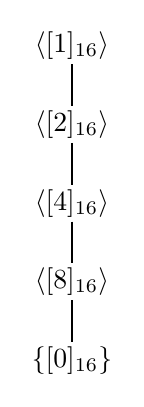
\begin{tikzpicture}[baseline=(current bounding box.center),every node/.style={inner sep=1.5pt}]
        \node (h16) at (0,0) {$\langle[1]_{16}\rangle$};
        \node (h8)  at (0,-1.0) {$\langle[2]_{16}\rangle$};
        \node (h4)  at (0,-2.0) {$\langle[4]_{16}\rangle$};
        \node (h2)  at (0,-3.0) {$\langle[8]_{16}\rangle$};
        \node (h1)  at (0,-4.0) {$\{[0]_{16}\}$};
        \draw (h16)--(h8)--(h4)--(h2)--(h1);
    \end{tikzpicture}
    \]

    \item
    \[
    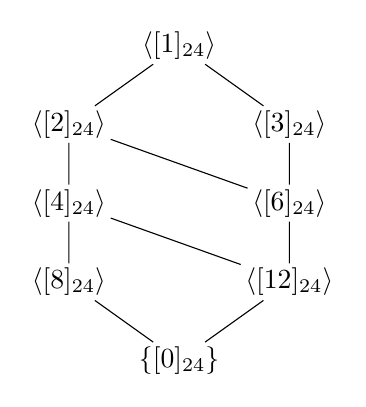
\begin{tikzpicture}[baseline=(current bounding box.center),every node/.style={inner sep=1.5pt}]
        \node (h24) at (0,0) {$\langle[1]_{24}\rangle$};
        \node (h12) at (-1.4,-1.0) {$\langle[2]_{24}\rangle$};
        \node (h8)  at (1.4,-1.0) {$\langle[3]_{24}\rangle$};
        \node (h6)  at (-1.4,-2.0) {$\langle[4]_{24}\rangle$};
        \node (h4)  at (1.4,-2.0) {$\langle[6]_{24}\rangle$};
        \node (h3)  at (-1.4,-3.0) {$\langle[8]_{24}\rangle$};
        \node (h2)  at (1.4,-3.0) {$\langle[12]_{24}\rangle$};
        \node (h1)  at (0,-4.0) {$\{[0]_{24}\}$};
        \draw (h24)--(h12) (h24)--(h8);
        \draw (h12)--(h6) (h12)--(h4) (h8)--(h4);
        \draw (h6)--(h3) (h6)--(h2) (h4)--(h2);
        \draw (h3)--(h1) (h2)--(h1);
    \end{tikzpicture}
    \]

    \item
    \[
    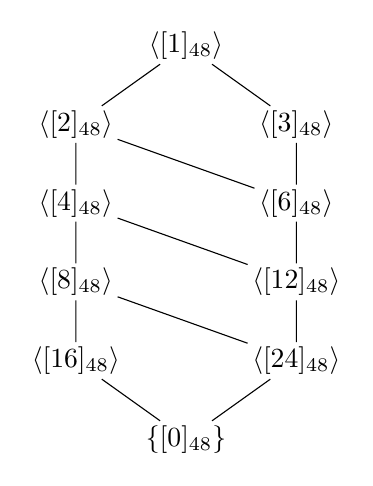
\begin{tikzpicture}[baseline=(current bounding box.center),every node/.style={inner sep=1.5pt}]
        \node (h48) at (0,0) {$\langle[1]_{48}\rangle$};
        \node (h24) at (-1.4,-1.0) {$\langle[2]_{48}\rangle$};
        \node (h16) at (1.4,-1.0) {$\langle[3]_{48}\rangle$};
        \node (h12) at (-1.4,-2.0) {$\langle[4]_{48}\rangle$};
        \node (h8)  at (1.4,-2.0) {$\langle[6]_{48}\rangle$};
        \node (h6)  at (-1.4,-3.0) {$\langle[8]_{48}\rangle$};
        \node (h4)  at (1.4,-3.0) {$\langle[12]_{48}\rangle$};
        \node (h3)  at (-1.4,-4.0) {$\langle[16]_{48}\rangle$};
        \node (h2)  at (1.4,-4.0) {$\langle[24]_{48}\rangle$};
        \node (h1)  at (0,-5.0) {$\{[0]_{48}\}$};
        \draw (h48)--(h24) (h48)--(h16);
        \draw (h24)--(h12) (h24)--(h8) (h16)--(h8);
        \draw (h12)--(h6) (h12)--(h4) (h8)--(h4);
        \draw (h6)--(h3) (h6)--(h2) (h4)--(h2);
        \draw (h3)--(h1) (h2)--(h1);
    \end{tikzpicture}
    \]
\end{exercisesubparts}
\end{solution}

\begin{exercise}{3.1.1}
Let $G$ and $H$ be groups. Let $\varphi\colon G\to H$ be a homomorphism and let $E$ be a subgroup of $H$. Prove that $\varphi^{-1}(E)\le G$, i.e., the preimage or pullback of a subgroup under a homomorphism is a subgroup. If $E\trianglelefteq H$, prove that $\varphi^{-1}(E)\trianglelefteq G$. Deduce that $\ker\varphi\trianglelefteq G$.
\end{exercise}

\begin{solution}
Since $\varphi(1_G)=1_H\in E$, the set $\varphi^{-1}(E)$ is nonempty. If $x,y\in\varphi^{-1}(E)$, then
\[
    \varphi(xy^{-1})=\varphi(x)\varphi(y)^{-1}\in E,
\]
so $xy^{-1}\in\varphi^{-1}(E)$. By the Subgroup Criterion,
\[
    \varphi^{-1}(E)\le G.
\]

Now suppose $E\trianglelefteq H$. If $g\in G$ and $x\in\varphi^{-1}(E)$, then
\[
    \varphi(gxg^{-1})
    =\varphi(g)\varphi(x)\varphi(g)^{-1}\in E,
\]
because $E$ is normal in $H$. Hence
\[
    \varphi^{-1}(E)\trianglelefteq G.
\]
Taking $E=\{1_H\}\trianglelefteq H$ gives
\[
    \ker\varphi=\varphi^{-1}(\{1_H\})\trianglelefteq G.
\]
\end{solution}

\begin{exercise}{3.1.2}
Let $\varphi\colon G\to H$ be a homomorphism of groups with kernel $K$, and let $a,b\in\varphi(G)$. Let $X\in G/K$ be the fiber above $a$ and let $Y$ be the fiber above $b$, i.e.,
\[
    X=\varphi^{-1}(a),
    \qquad
    Y=\varphi^{-1}(b).
\]
Fix an element $u\in X$, so $\varphi(u)=a$. Prove that if $XY=Z$ in the quotient group $G/K$ and $w$ is any member of $Z$, then there is some $y\in Y$ such that $uy=w$.
\end{exercise}

\begin{hint}
Show that $u^{-1}w\in Y$.
\end{hint}

\begin{solution}
By the description of fibers in $\S3.1$, $X=uK$. Choose $v\in Y$, so $Y=vK$. Since
\[
    Z=XY=(uK)(vK)=uvK,
\]
any $w\in Z$ has the form
\[
    w=uvk
\]
for some $k\in K$. Set
\[
    y=u^{-1}w=vk.
\]
Since $vk\in vK=Y$, we have $y\in Y$, and by construction
\[
    uy=w.
\]
\end{solution}

\begin{exercise}{3.1.7}
Define $\pi\colon\R^2\to\R$ by
\[
    \pi((x,y))=x+y.
\]
Prove that $\pi$ is a surjective homomorphism and describe the kernel and fibers of $\pi$ geometrically.
\end{exercise}

\begin{solution}
For $(x_1,y_1),(x_2,y_2)\in\R^2$,
\[
\begin{aligned}
    \pi((x_1,y_1)+(x_2,y_2))
    &=\pi((x_1+x_2,y_1+y_2))\\
    &=x_1+x_2+y_1+y_2\\
    &=\pi((x_1,y_1))+\pi((x_2,y_2)).
\end{aligned}
\]
Thus $\pi$ is a homomorphism. It is surjective because for every $c\in\R$,
\[
    \pi((c,0))=c.
\]

The kernel is
\[
    \ker\pi
    =\{(x,y)\in\R^2\mid x+y=0\}
    =\{(t,-t)\mid t\in\R\},
\]
the line through the origin with slope $-1$. More generally, the fiber above $c\in\R$ is
\[
    \pi^{-1}(c)
    =\{(x,y)\in\R^2\mid x+y=c\},
\]
which is the line of slope $-1$ with $y$-intercept $c$. Hence the fibers are parallel affine lines, each a coset of $\ker\pi$.
\end{solution}

\end{document}
